\subsection*{Problema 13}

\textbf{Enunciado:} Calcular la integral:
\begin{equation*}
\int \frac{\sin x \, dx}{1 + \sin x + \cos x}
\end{equation*}

\textbf{Solución:} Para resolver la integral trigonométrica, aplicamos la sustitución universal de Weierstrass, definida como:
\begin{equation*}
z = \tan\left(\frac{x}{2}\right)
\end{equation*}

De esta sustitución, las identidades trigonométricas fundamentales y el diferencial se expresan de la siguiente manera:
\begin{align*}
\sin x &= \dfrac{2z}{1 + z^2}, \quad 
\cos x = \dfrac{1 - z^2}{1 + z^2} \\
dx &= \dfrac{2 \, dz}{1 + z^2}
\end{align*}

Sustituimos estas expresiones en la integral original del problema:
\begin{align*}
&\int \dfrac{\frac{2z}{1 + z^2}}{1 + \frac{2z}{1 + z^2} + \frac{1 - z^2}{1 + z^2}} \cdot \dfrac{2 \, dz}{1 + z^2} \\
&= \int \dfrac{\frac{2z}{1 + z^2}}{\frac{1 + z^2 + 2z + 1 - z^2}{1 + z^2}} \cdot \dfrac{2 \, dz}{1 + z^2}
\end{align*}

Simplificando el denominador y cancelando términos semejantes, obtenemos:
\begin{align*}
&= \int \dfrac{2z}{2 + 2z} \cdot \dfrac{2 \, dz}{1 + z^2} \\
&= \int \dfrac{z}{1 + z} \cdot \dfrac{2 \, dz}{1 + z^2} \\
&= 2 \int \dfrac{z \, dz}{(1 + z)(1 + z^2)}
\end{align*}

Descomponemos el integrando en fracciones parciales de la siguiente forma:
\begin{align*}
\dfrac{z}{(1 + z)(1 + z^2)} &= \dfrac{A}{1 + z} + \dfrac{Bz + C}{1 + z^2}
\end{align*}

Multiplicando ambos lados por el denominador común:
\begin{equation*}
z = A(1 + z^2) + (Bz + C)(1 + z)
\end{equation*}

Evaluamos en valores convenientes de $z$ para hallar las constantes:
\begin{align*}
\text{Si } z &= -1: \\
-1 &= A(1 + (-1)^2) \implies 2A = -1 \implies A = -\dfrac{1}{2}
\end{align*}

Igualando coeficientes para las potencias de $z$:
\begin{align*}
\text{Para } z^2: &\quad 0 = A + B \implies B = \dfrac{1}{2} \\
\text{Para } z^0: &\quad 0 = A + C \implies C = \dfrac{1}{2}
\end{align*}

Sustituimos las constantes encontradas en la descomposición:
\begin{align*}
\int &\dfrac{z \, dz}{(1 + z)(1 + z^2)} = \\
&\int \left( \dfrac{-1/2}{1 + z} + \dfrac{\frac{1}{2}z + \frac{1}{2}}{1 + z^2} \right) dz
\end{align*}

Integramos cada término por separado:
\begin{align*}
&= -\dfrac{1}{2} \ln|1 + z| + \dfrac{1}{4} \ln(1 + z^2) \\
&\quad + \dfrac{1}{2} \arctan(z) + C_1
\end{align*}

Multiplicando por el factor $2$ inicial:
\begin{align*}
&= -\ln|1 + z| + \dfrac{1}{2} \ln(1 + z^2) + \arctan(z) + C
\end{align*}

Regresando a la variable original $x$ mediante $z = \tan(x/2)$ y utilizando propiedades logarítmicas:
\begin{align*}
\int &\dfrac{\sin x \, dx}{1 + \sin x + \cos x} = \\
&\ln\left|\dfrac{\sqrt{1 + \tan^2(x/2)}}{1 + \tan(x/2)}\right| + \dfrac{x}{2} + C
\end{align*}
Simplificando el argumento, el resultado final es:
\begin{equation*}
x - \ln\left|1 + \tan\left(\frac{x}{2}\right)\right| - \ln\left(\cos\left(\frac{x}{2}\right)\right) + C
\end{equation*}

\begin{figure}[H]
	\centering
	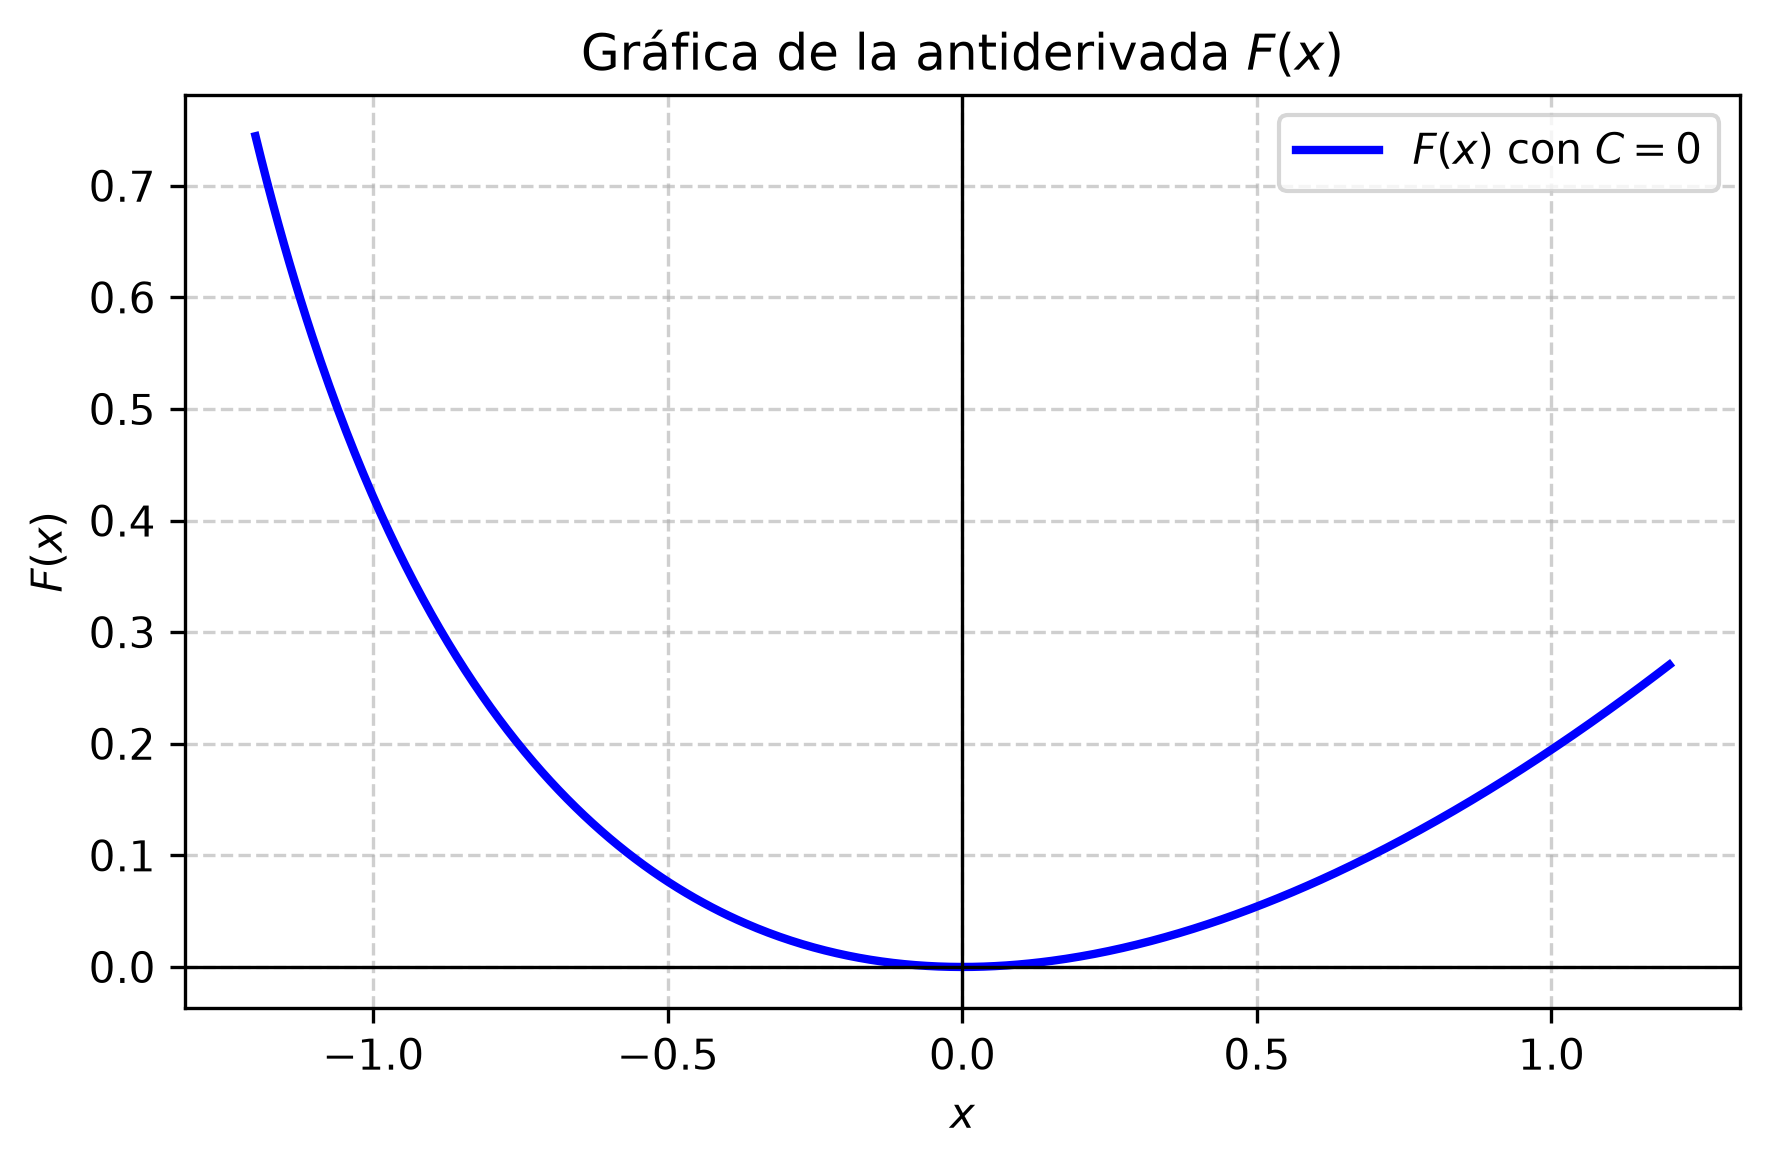
\includegraphics[width=\columnwidth]{semana_04/graficas/SEM04_P13_grafica.png}
	\caption{Representación gráfica de $f(x)$ y su antiderivada $F(x)$ evaluada para la constante de integración $C = 0$ (Problema 13).}
	\label{fig:problema13}
\end{figure}
